\section{Introduction}

The legal profession increasingly relies on artificial intelligence to manage the growing complexity and volume of legal documents, particularly in contract review and analysis. Traditional manual contract review is time-intensive, error-prone, and costly, creating a significant bottleneck in legal practice \cite{katz2017general}. While machine learning has shown promise in legal applications \cite{zhong2018legal, sulea2017exploring}, the deployment of AI systems in high-stakes legal environments demands not only accuracy but also transparency and interpretability.

Recent advances in transformer-based models have demonstrated remarkable capabilities in legal natural language processing tasks. The Contract Understanding Atticus Dataset (CUAD) \cite{hendrycks2021cuad} provides a comprehensive benchmark for legal clause extraction, containing 510 legal contracts annotated for 41 different clause types. Specialized legal language models such as Legal-BERT \cite{chalkidis2020legal} have shown superior performance on legal text understanding compared to general-purpose models, while modern text-to-text transformers like T5 \cite{raffel2020t5} enable sophisticated document summarization capabilities.

However, the application of AI in legal contexts faces a critical challenge: the "black box" nature of deep learning models undermines trust and adoption among legal practitioners who require transparent, interpretable decision-making processes. The legal domain's emphasis on precedent, reasoning, and accountability necessitates explainable AI (XAI) approaches that can provide clear justifications for model predictions \cite{molnar2020interpretable}. Methods such as SHAP (SHapley Additive exPlanations) \cite{lundberg2017unified} offer principled approaches to model interpretability, enabling legal professionals to understand and validate AI-driven insights.

Furthermore, legal document analysis presents unique technical challenges that distinguish it from general NLP tasks. As illustrated in Figure \ref{fig:clause_presence_distribution}, my analysis of the CUAD dataset reveals severe class imbalance, with only 32.1\% of questions having corresponding clauses present across all document types. This imbalance is further exemplified in Figure \ref{fig:clause_presence_frequency}, which shows the dramatic variation in clause frequencies, with nine clause types appearing in fewer than 10\% of documents while others like "Document Name" appear universally. The multi-label nature of legal clause detection \cite{liu2021multilabel}, combined with the specialized legal terminology and long document contexts (mean length ~4,800 characters as shown in Figure \ref{fig:context_lengths_distribution}), requires careful model design and evaluation approaches.

\begin{figure}[htbp]
\centering
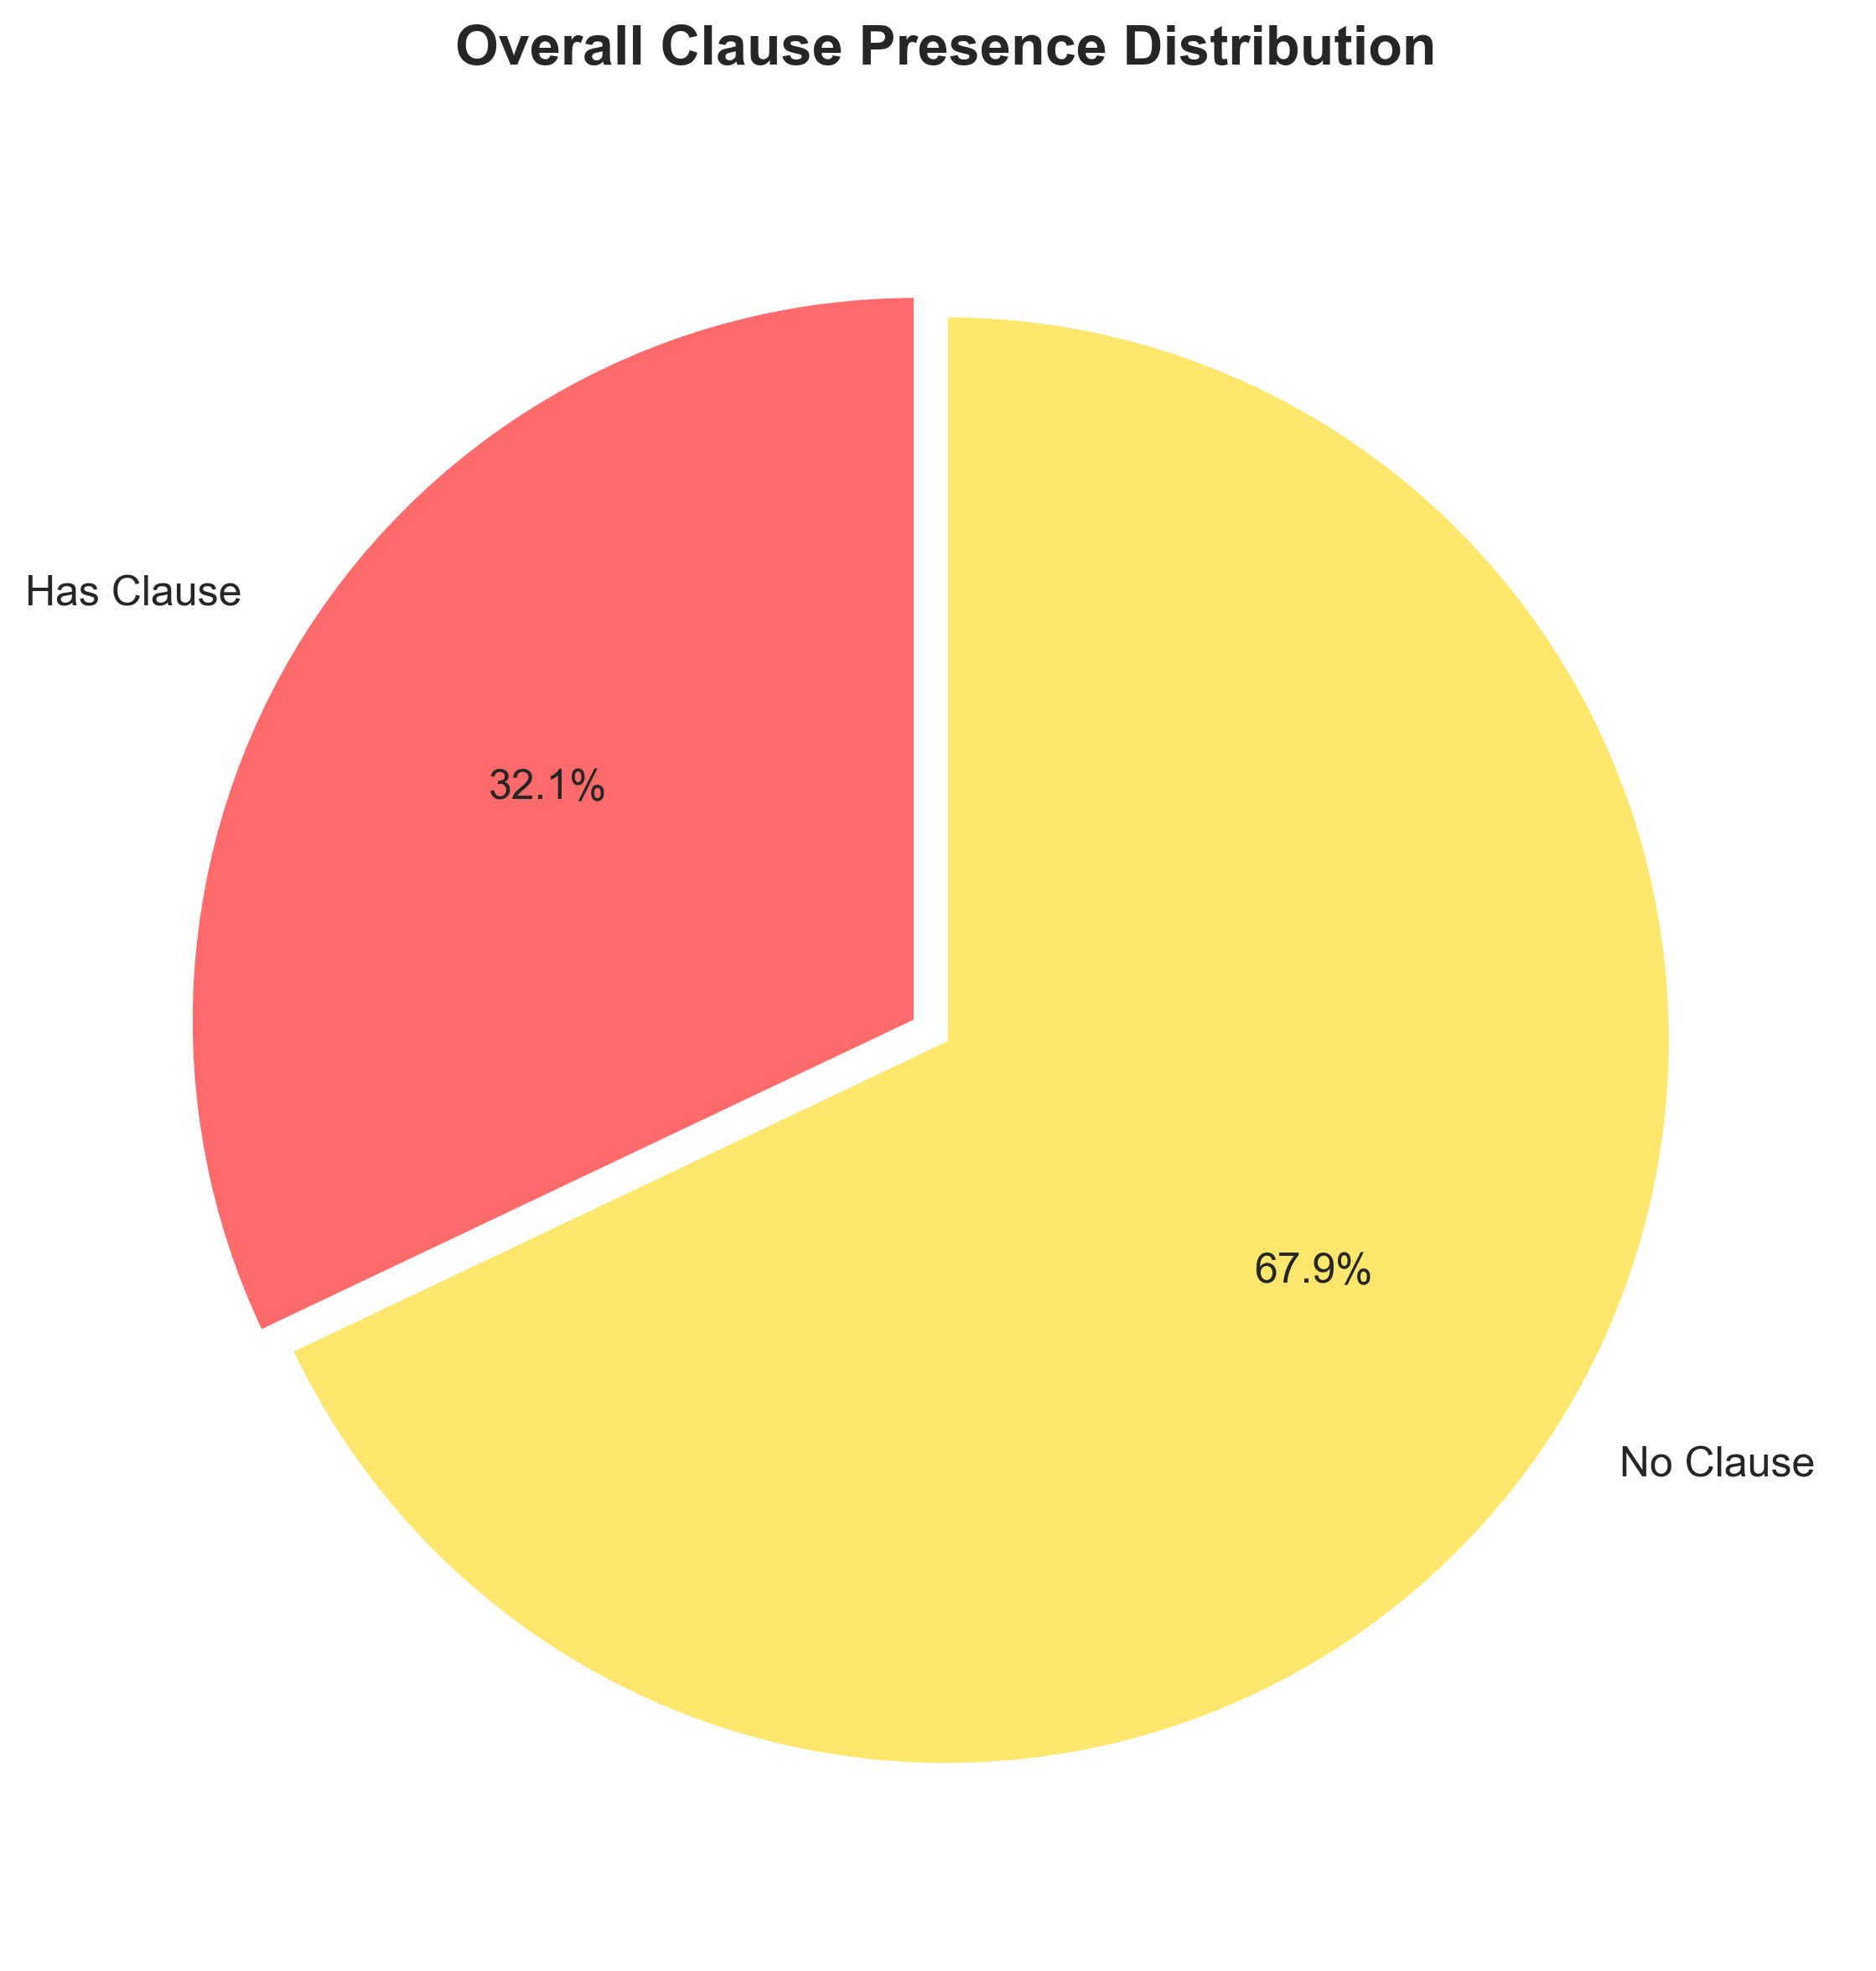
\includegraphics[width=0.45\textwidth]{../figures/clause_presence_distribution.png}
\caption{Overall distribution of clause presence vs. absence in the CUAD dataset, showing severe class imbalance with only 32.1\% positive instances.}
\label{fig:clause_presence_distribution}
\end{figure}

\begin{figure}[htbp]
\centering
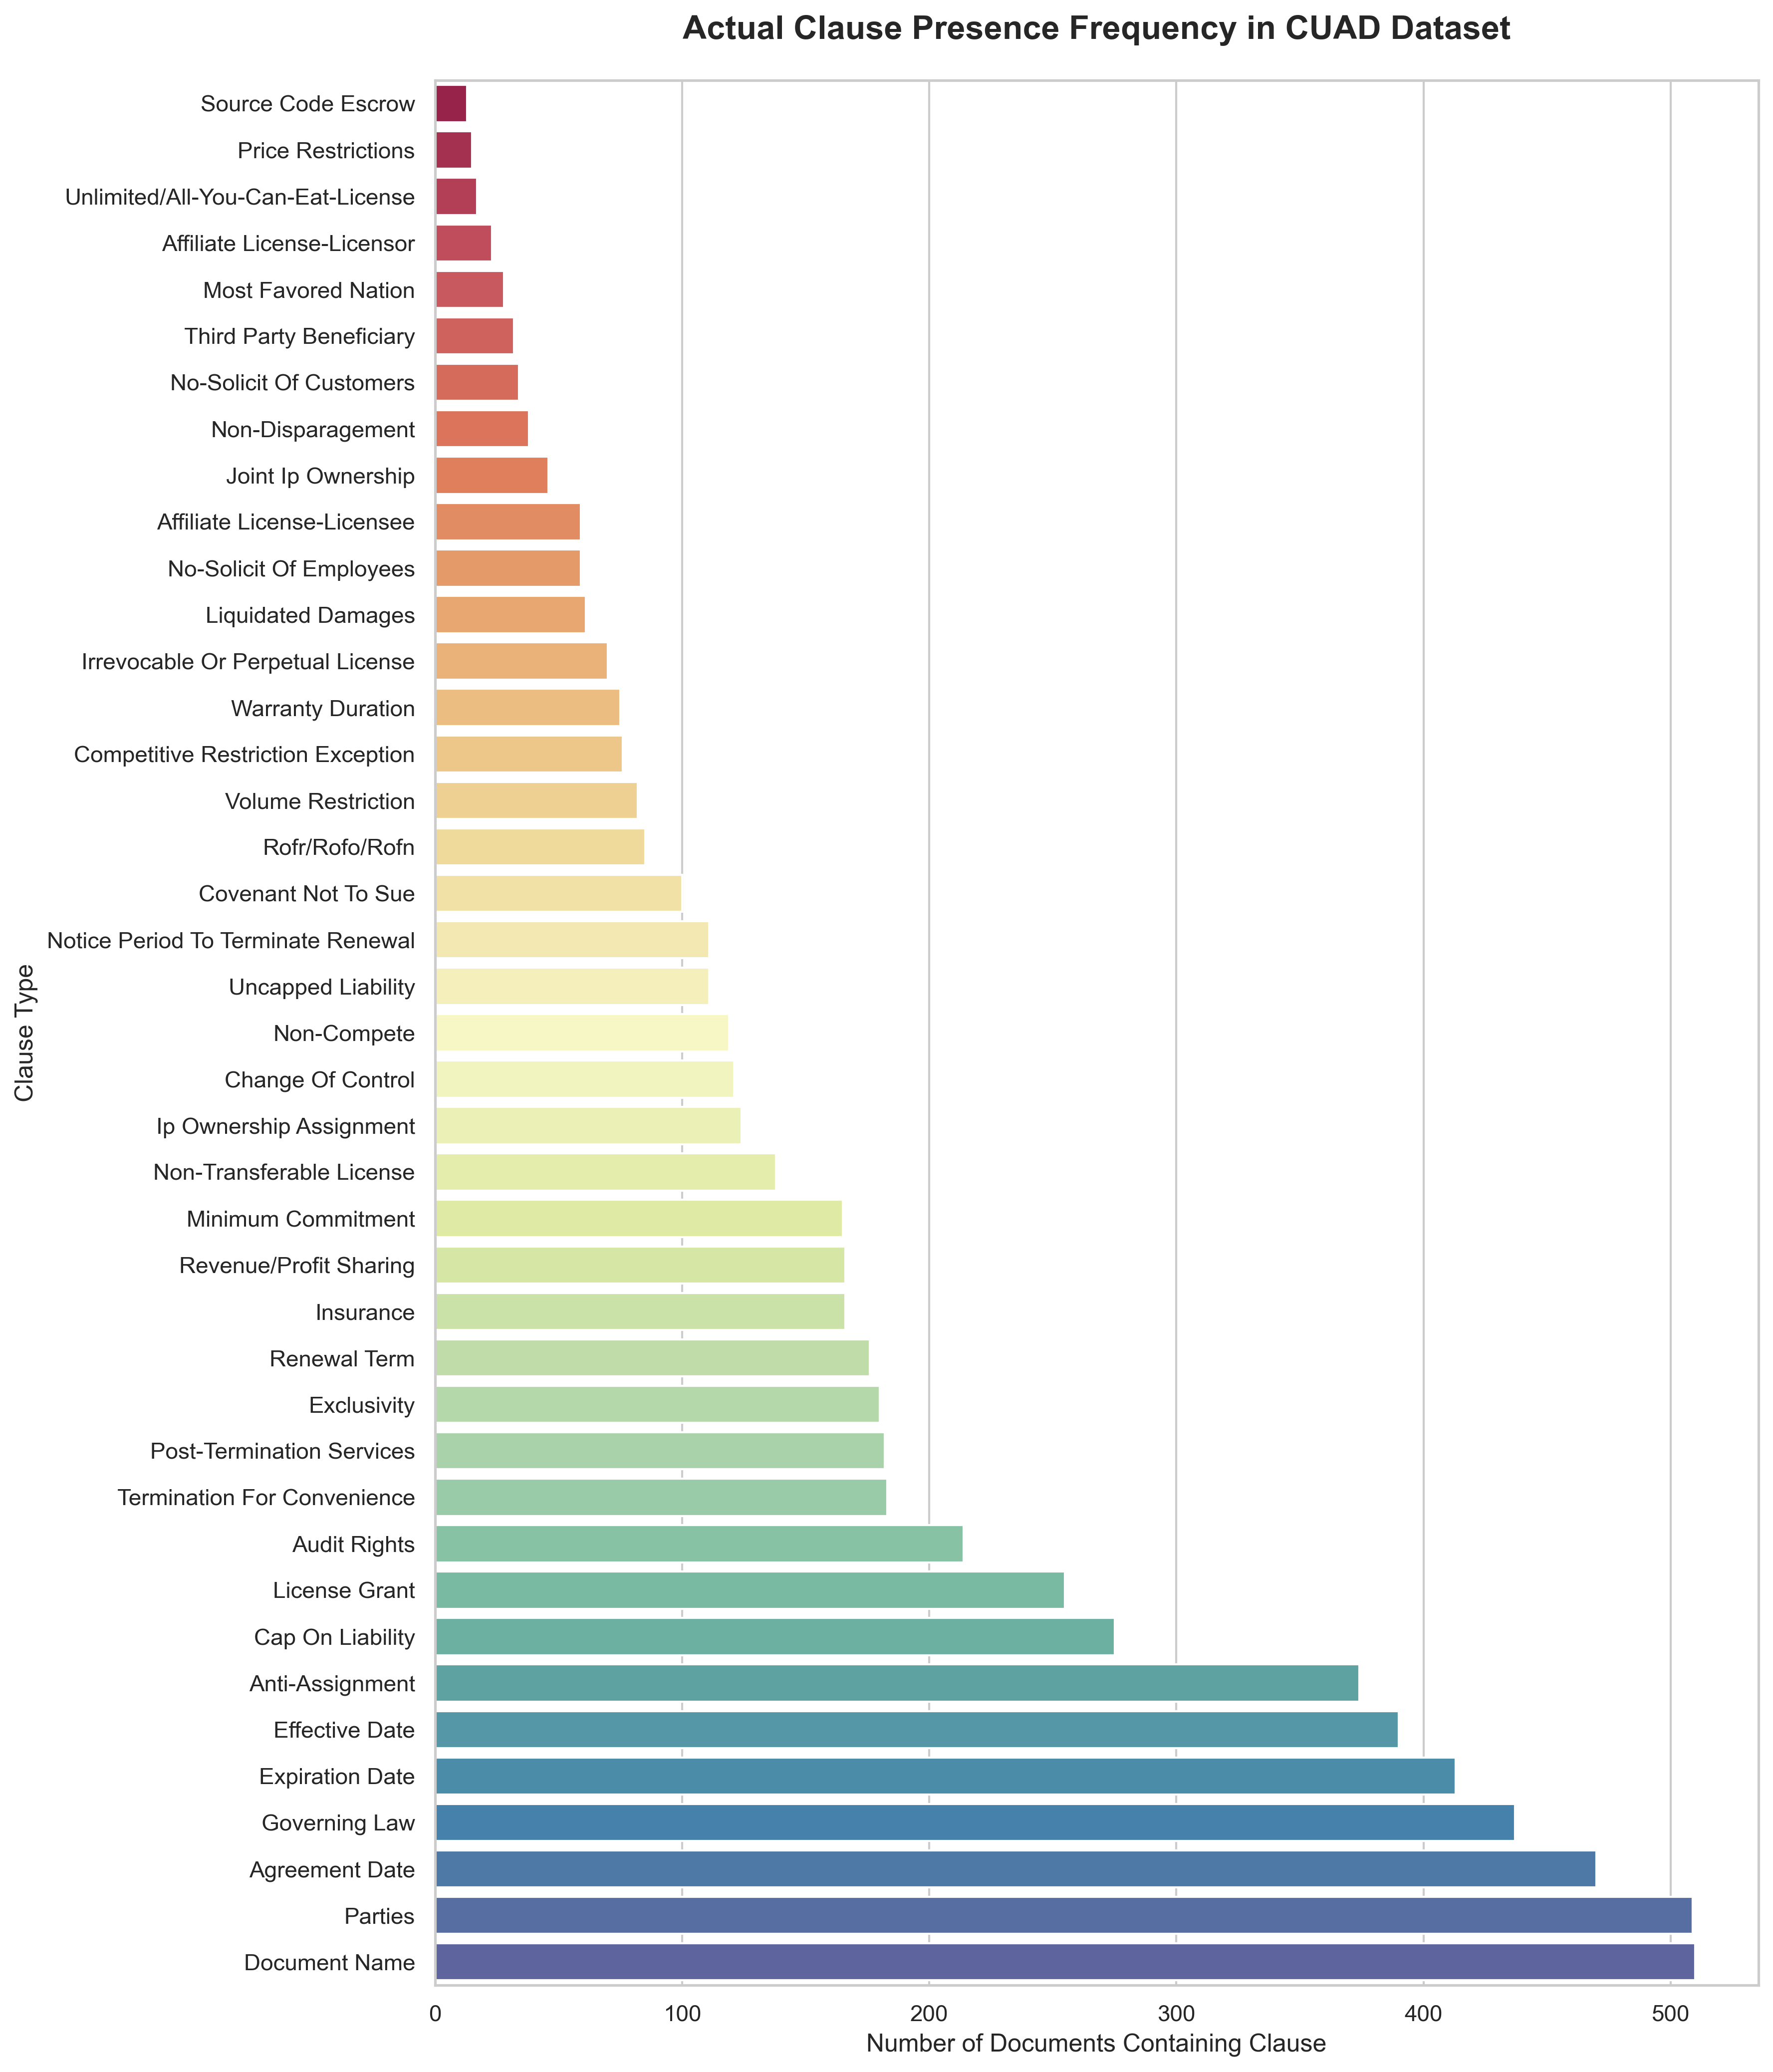
\includegraphics[width=0.48\textwidth]{../figures/clause_presence_frequency.png}
\caption{Frequency distribution of clause types in CUAD dataset, demonstrating extreme variability from universal presence (Document Name) to rare occurrences (<10\% for nine clause types).}
\label{fig:clause_presence_frequency}
\end{figure}

\begin{figure}[htbp]
\centering
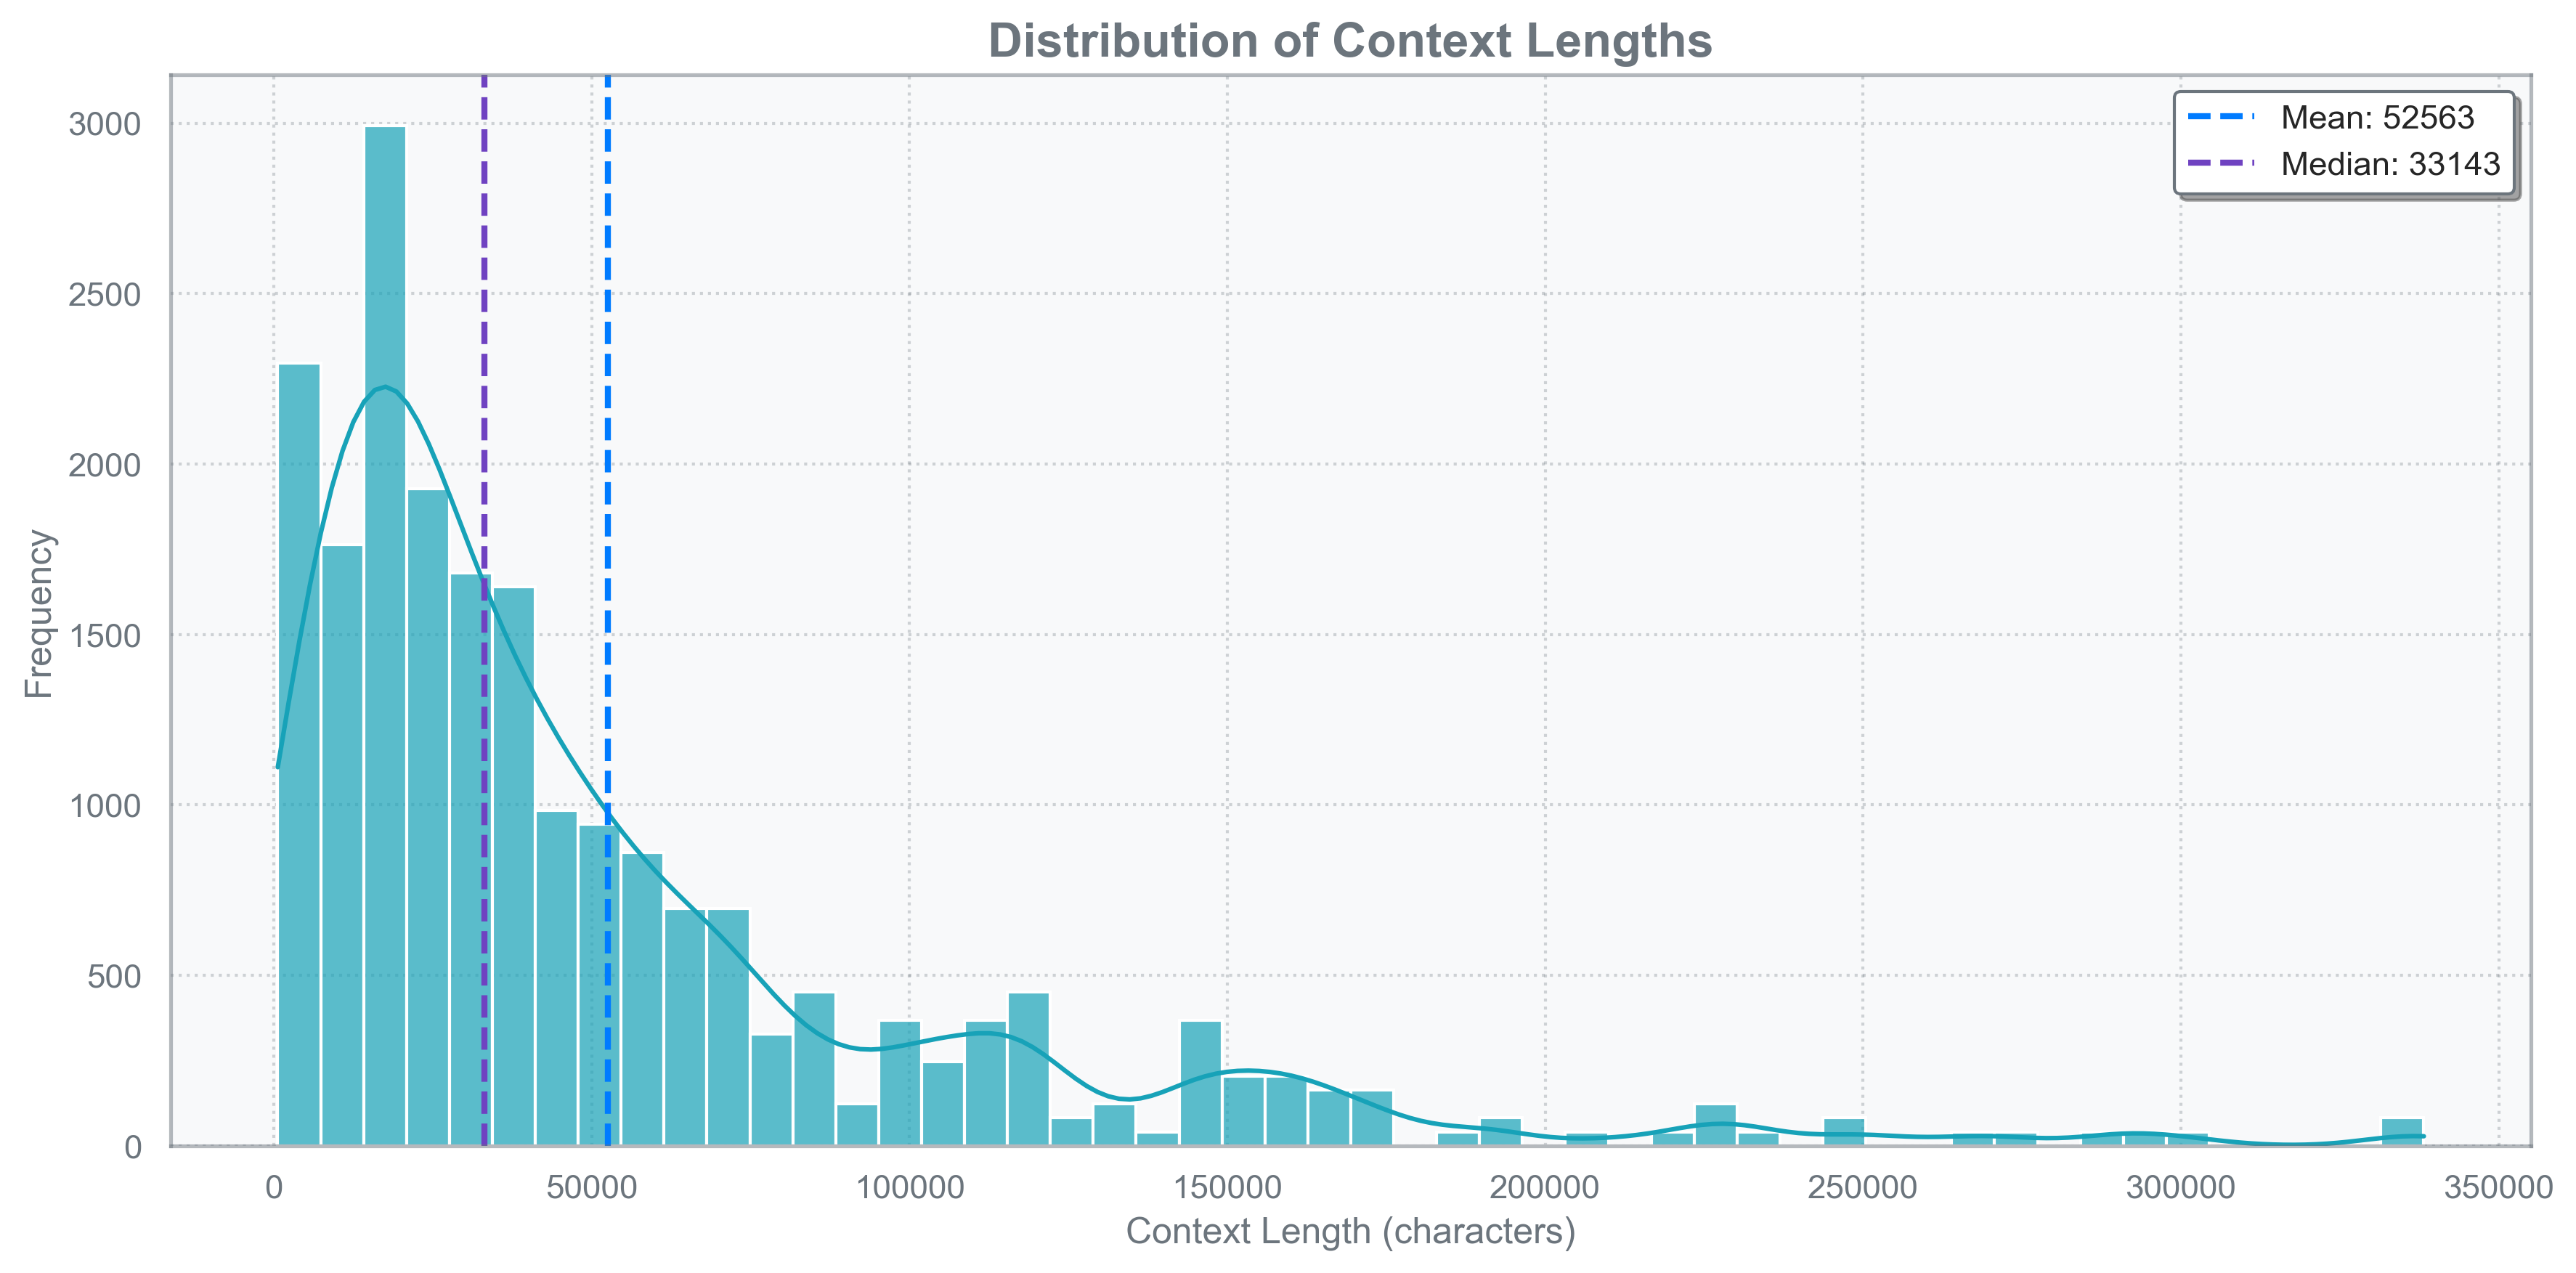
\includegraphics[width=0.45\textwidth]{../figures/context_lengths_distribution.png}
\caption{Distribution of context lengths in legal documents, showing the challenge of processing long sequences with mean length of approximately 4,800 characters.}
\label{fig:context_lengths_distribution}
\end{figure}

The deployment of machine learning systems in legal practice also faces significant practical challenges \cite{paleyes2022challenges}, including model reliability, data privacy, regulatory compliance, and integration with existing legal workflows. These considerations are particularly critical in legal applications where model failures can have serious professional and financial consequences.

This paper presents a comprehensive approach to interpretable legal document analysis that addresses these challenges through: (1) multi-label clause extraction using domain-specialized BERT models fine-tuned on legal text, (2) abstractive legal document summarization with T5-based architectures, and (3) integrated explainability features using SHAP analysis and attention visualization to provide transparent, actionable insights for legal practitioners.

My contributions include: a complete end-to-end pipeline for legal document analysis with integrated explainability, comprehensive evaluation on the CUAD dataset demonstrating the impact of class imbalance on model performance, and practical deployment considerations for AI systems in legal practice. Through this work, I aim to bridge the gap between advanced NLP capabilities and the practical requirements of legal professionals, advancing the responsible adoption of AI in legal technology.

